%\newsection{Kapitel1}

%Hier den Inhalt mit \input einfügen und die folgenden Zeilen entfernen

%%%%% Fuer Widerstandstabelle
\definecolor{gold}{RGB}{255, 210, 0}
\definecolor{silver}{RGB}{192, 192, 192}
\definecolor{brown}{RGB} {138, 80, 45}

%%%% -----------------


	\section{Leitfähigkeit und Widerstand}
\begin{frame}
	\ftx{Lernziele: Leitfähigkeit und Widerstand}
\b{
	\begin{Lernziele}{Leitfähigkeit und Widerstand} % ToDo: Temperaturabhängigkeit ersetzen durch nur Temperatur (in den Items bereits passiert, weiter noch nicht geprüft)
		Die Studierenden
		\begin{itemize}
		\item kennen das elektrische Bauelement Widerstand.
		\item können die unterschiedlichen Bauteilausführungen von Widerständen erklären.
		\item können anhand des spezifischen Widerstand $\rho$ oder des spezifischen Leitwertes $\kappa$ Berechnungen durchführen.
		\item können die Unterschiede in der Leitfähigkeit verschiedener Materialien basierend auf deren atomarer Struktur und Temperatur analysieren.
	\end{itemize}
	\end{Lernziele}
}
\speech{text}{1}{
In dem nun folgenden Abschnitt des Moduls werden wir uns mit der Leitfähigkeit und dem Widerstand beschäftigen. 
Sie sollten am Ende dieses Abschnittes den elektrischen Widerstand als Bauelement kennen und auch seine Eigenschaften. 
Sie kennen unterschiedliche Bauteilausführungen von Widerstand und können diese auch erläutern. 
Ferner ist es Ihnen möglich, anhand des spezifischen Widerstandes oder des spezifischen Leitwertes Berechnungen durchführen zu können, z.B. den Widerstand einer Anordnung berechnen. 
Und Sie können die Unterschiede der Leitfähigkeit in verschiedenen Materialien basierend auf der atomaren Struktur und der Temperatur analysieren.
}

\end{frame}
\begin{frame}
	\ftx{Leitfähigkeit und Widerstand}
\s{% nur im Skript
Die Leitfähigkeit oder auch der Leitwert $G$ beschreibt, wie der Name schon impliziert, die Fähigkeit eines Materials elektrischen Strom zu leiten. 
Je größer der Wert, desto besser leitet ein Material, sprich, umso einfacher können sich die Ladungsträger im Material bewegen. 
Diese Eigenschaft basiert auf den Experimenten eines deutschen Experimentalphysikers Georg Simon Ohm anfang des 19. Jahrhunderts, 
in welchen er herausfand, dass sich der Strom proportional zur angelegten Spannung verhält. 
Der Kehrwert des Leitwertes ist der heute gebräuchlichere ohm'sche Widerstand $R$. 
Der Leitwert $G$ hat die Einheit Siemens (S), der ohmsche Widerstand die Einheit Ohm ($\Omega$).
}% nur im Skript

%%%%%%%%%%%%%%%%%%%%%%%%%%%%%%%%%%%%%%%%%%%% Formeln - Ohm´sches Gesetz %%%%%%%%%%%%%%%%%%%%%%%%%%%%%%%%%%%%%

% \begin{equation}
% 	I = G \cdot U 
% \end{equation}

% \begin{equation}
% 	U = R \cdot I 
% \end{equation}

%%%%%%%%%%%%%%%%%%%%%%%%%%%%%%%%%%%%%%%%%%%% Ende: Formeln - Ohm´sches Gesetz %%%%%%%%%%%%%%%%%%%%%%%%%%%%%%%%%%%%%
%%%%%%%%%%%%%%%%%%%%%%%%%%%%%%%%%%%%%%%%%%%%% Anfang - Abbildung Widerstände %%%%%%%%%%%%%%%%%%%%%%%%%%%%%%%%%%%%
\b{
	\begin{itemize}
		\item Unterschiedliche Bauteilausführungen von Widerständen
	\end{itemize}
}

	\begin{figure}[H]
		\centering
		\b{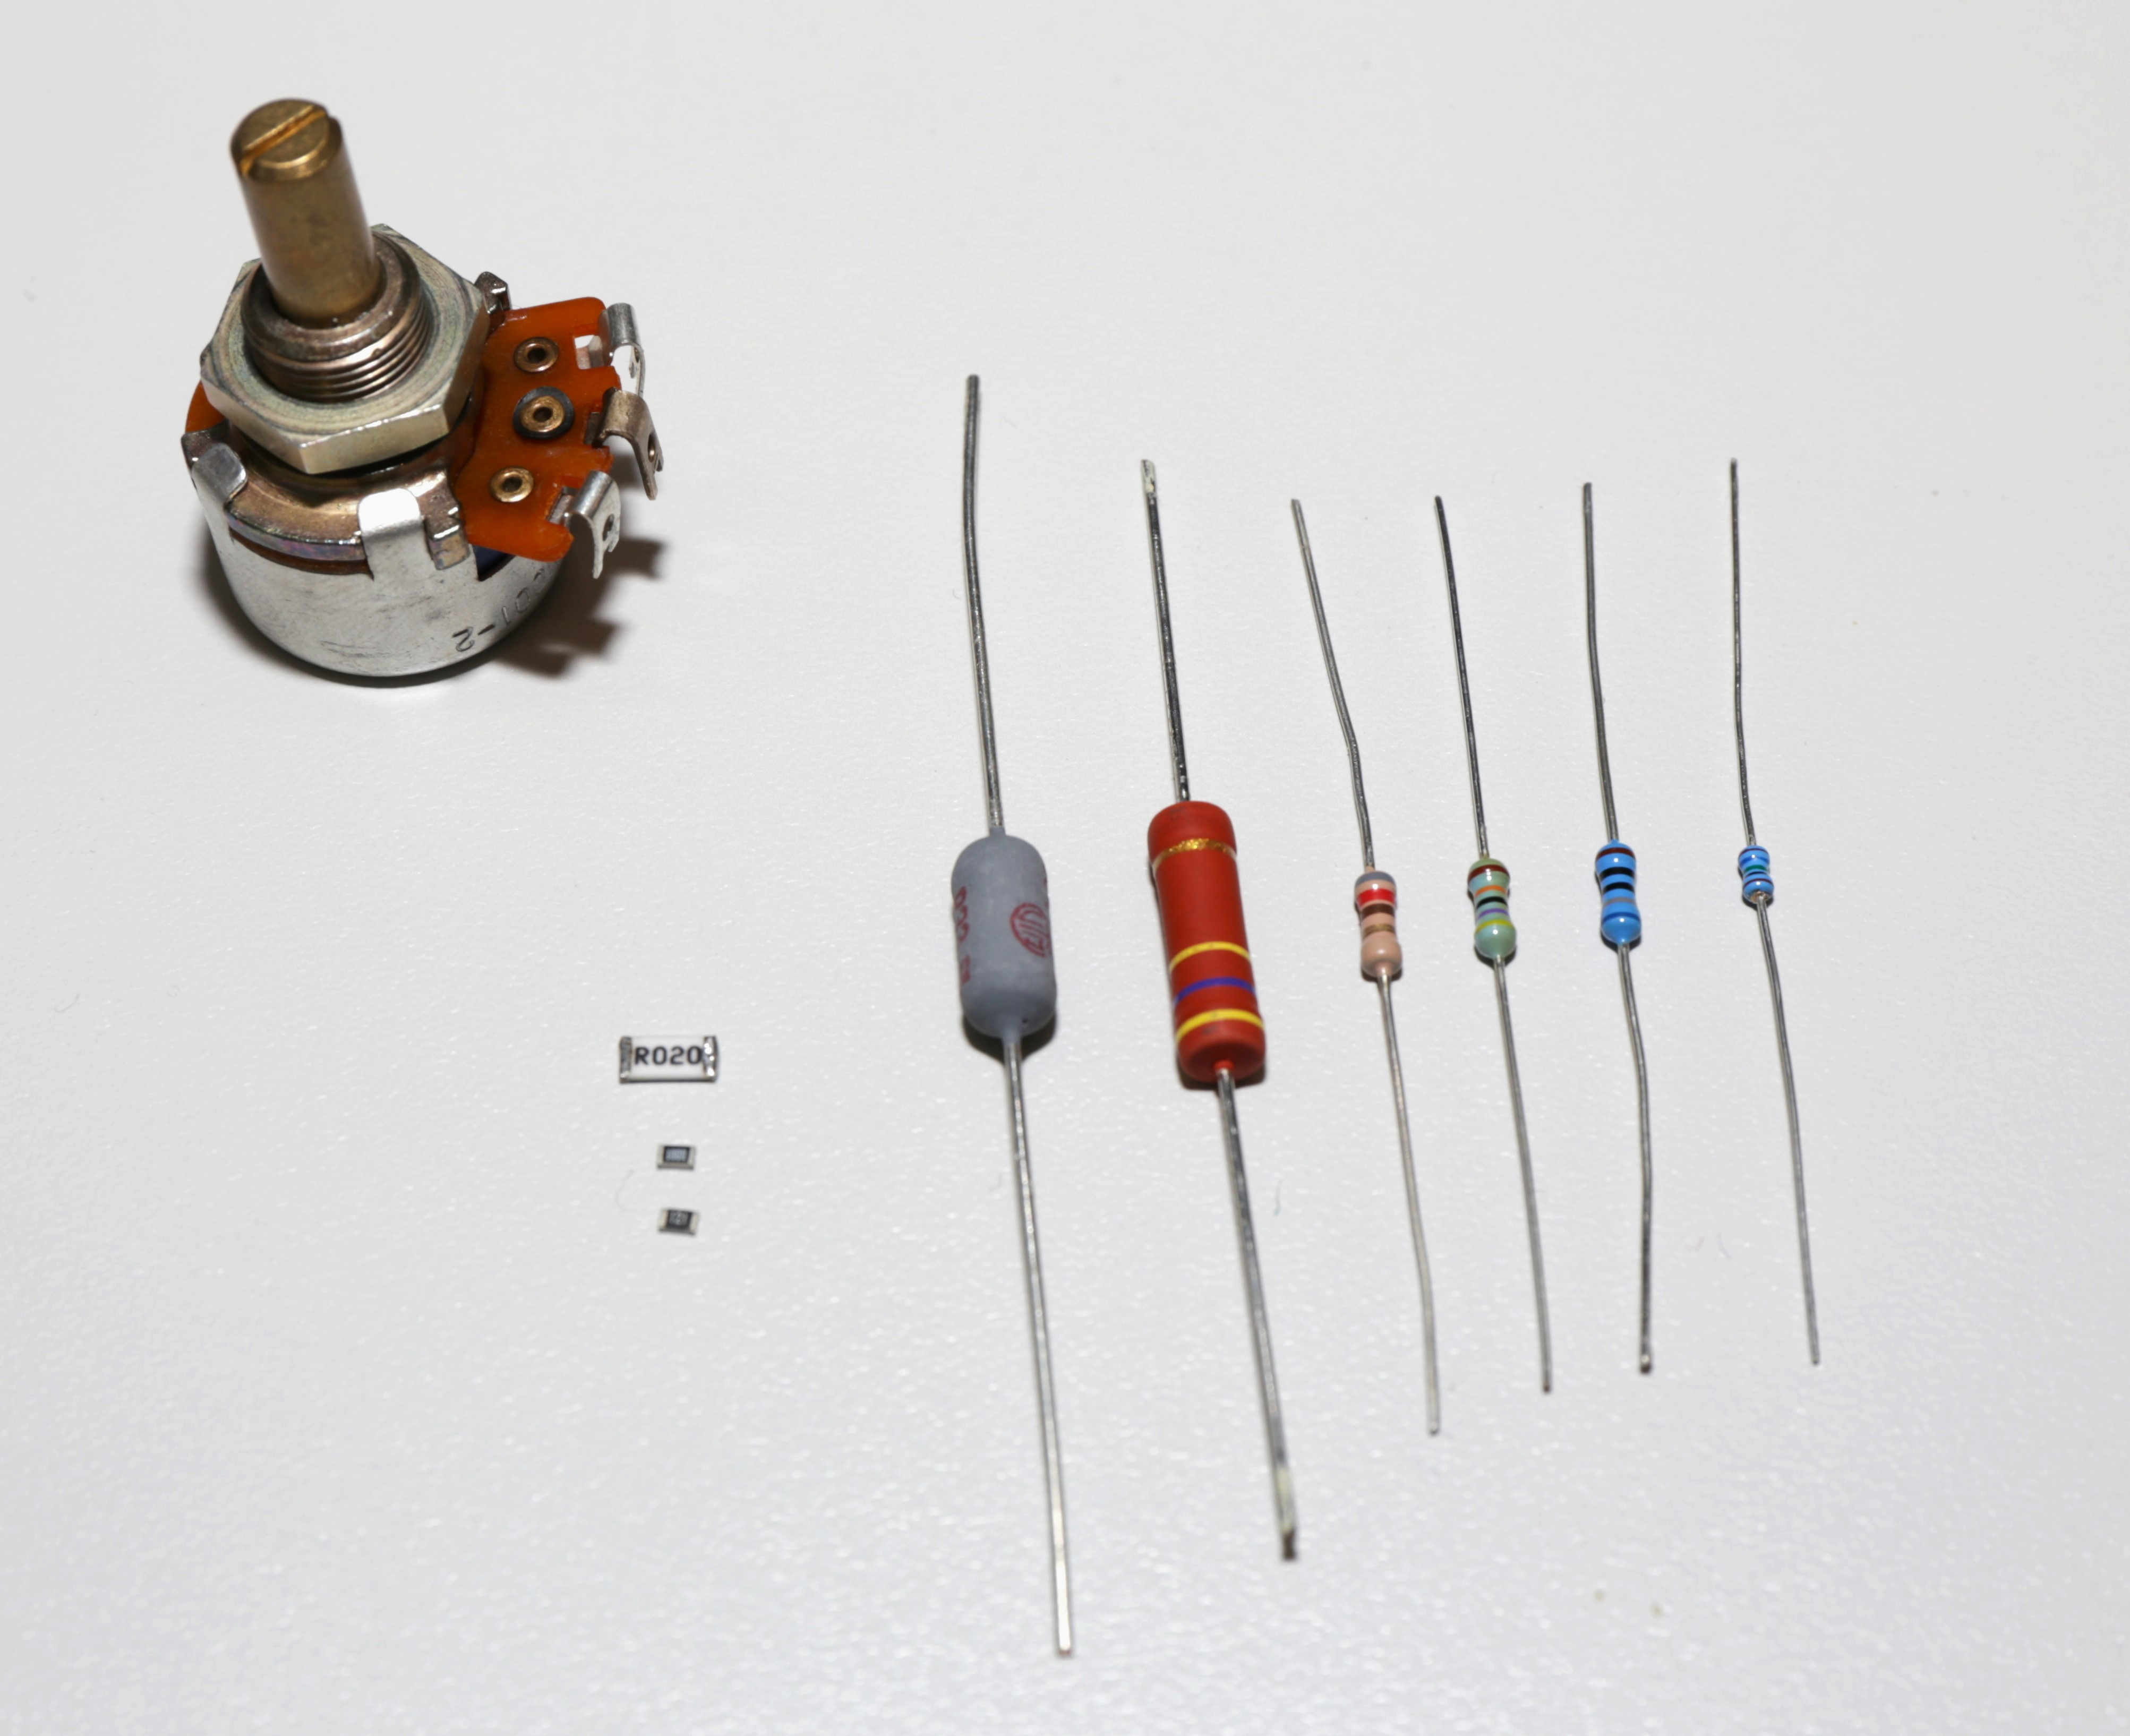
\includegraphics[width=0.45\textwidth]{wi}}
		\s{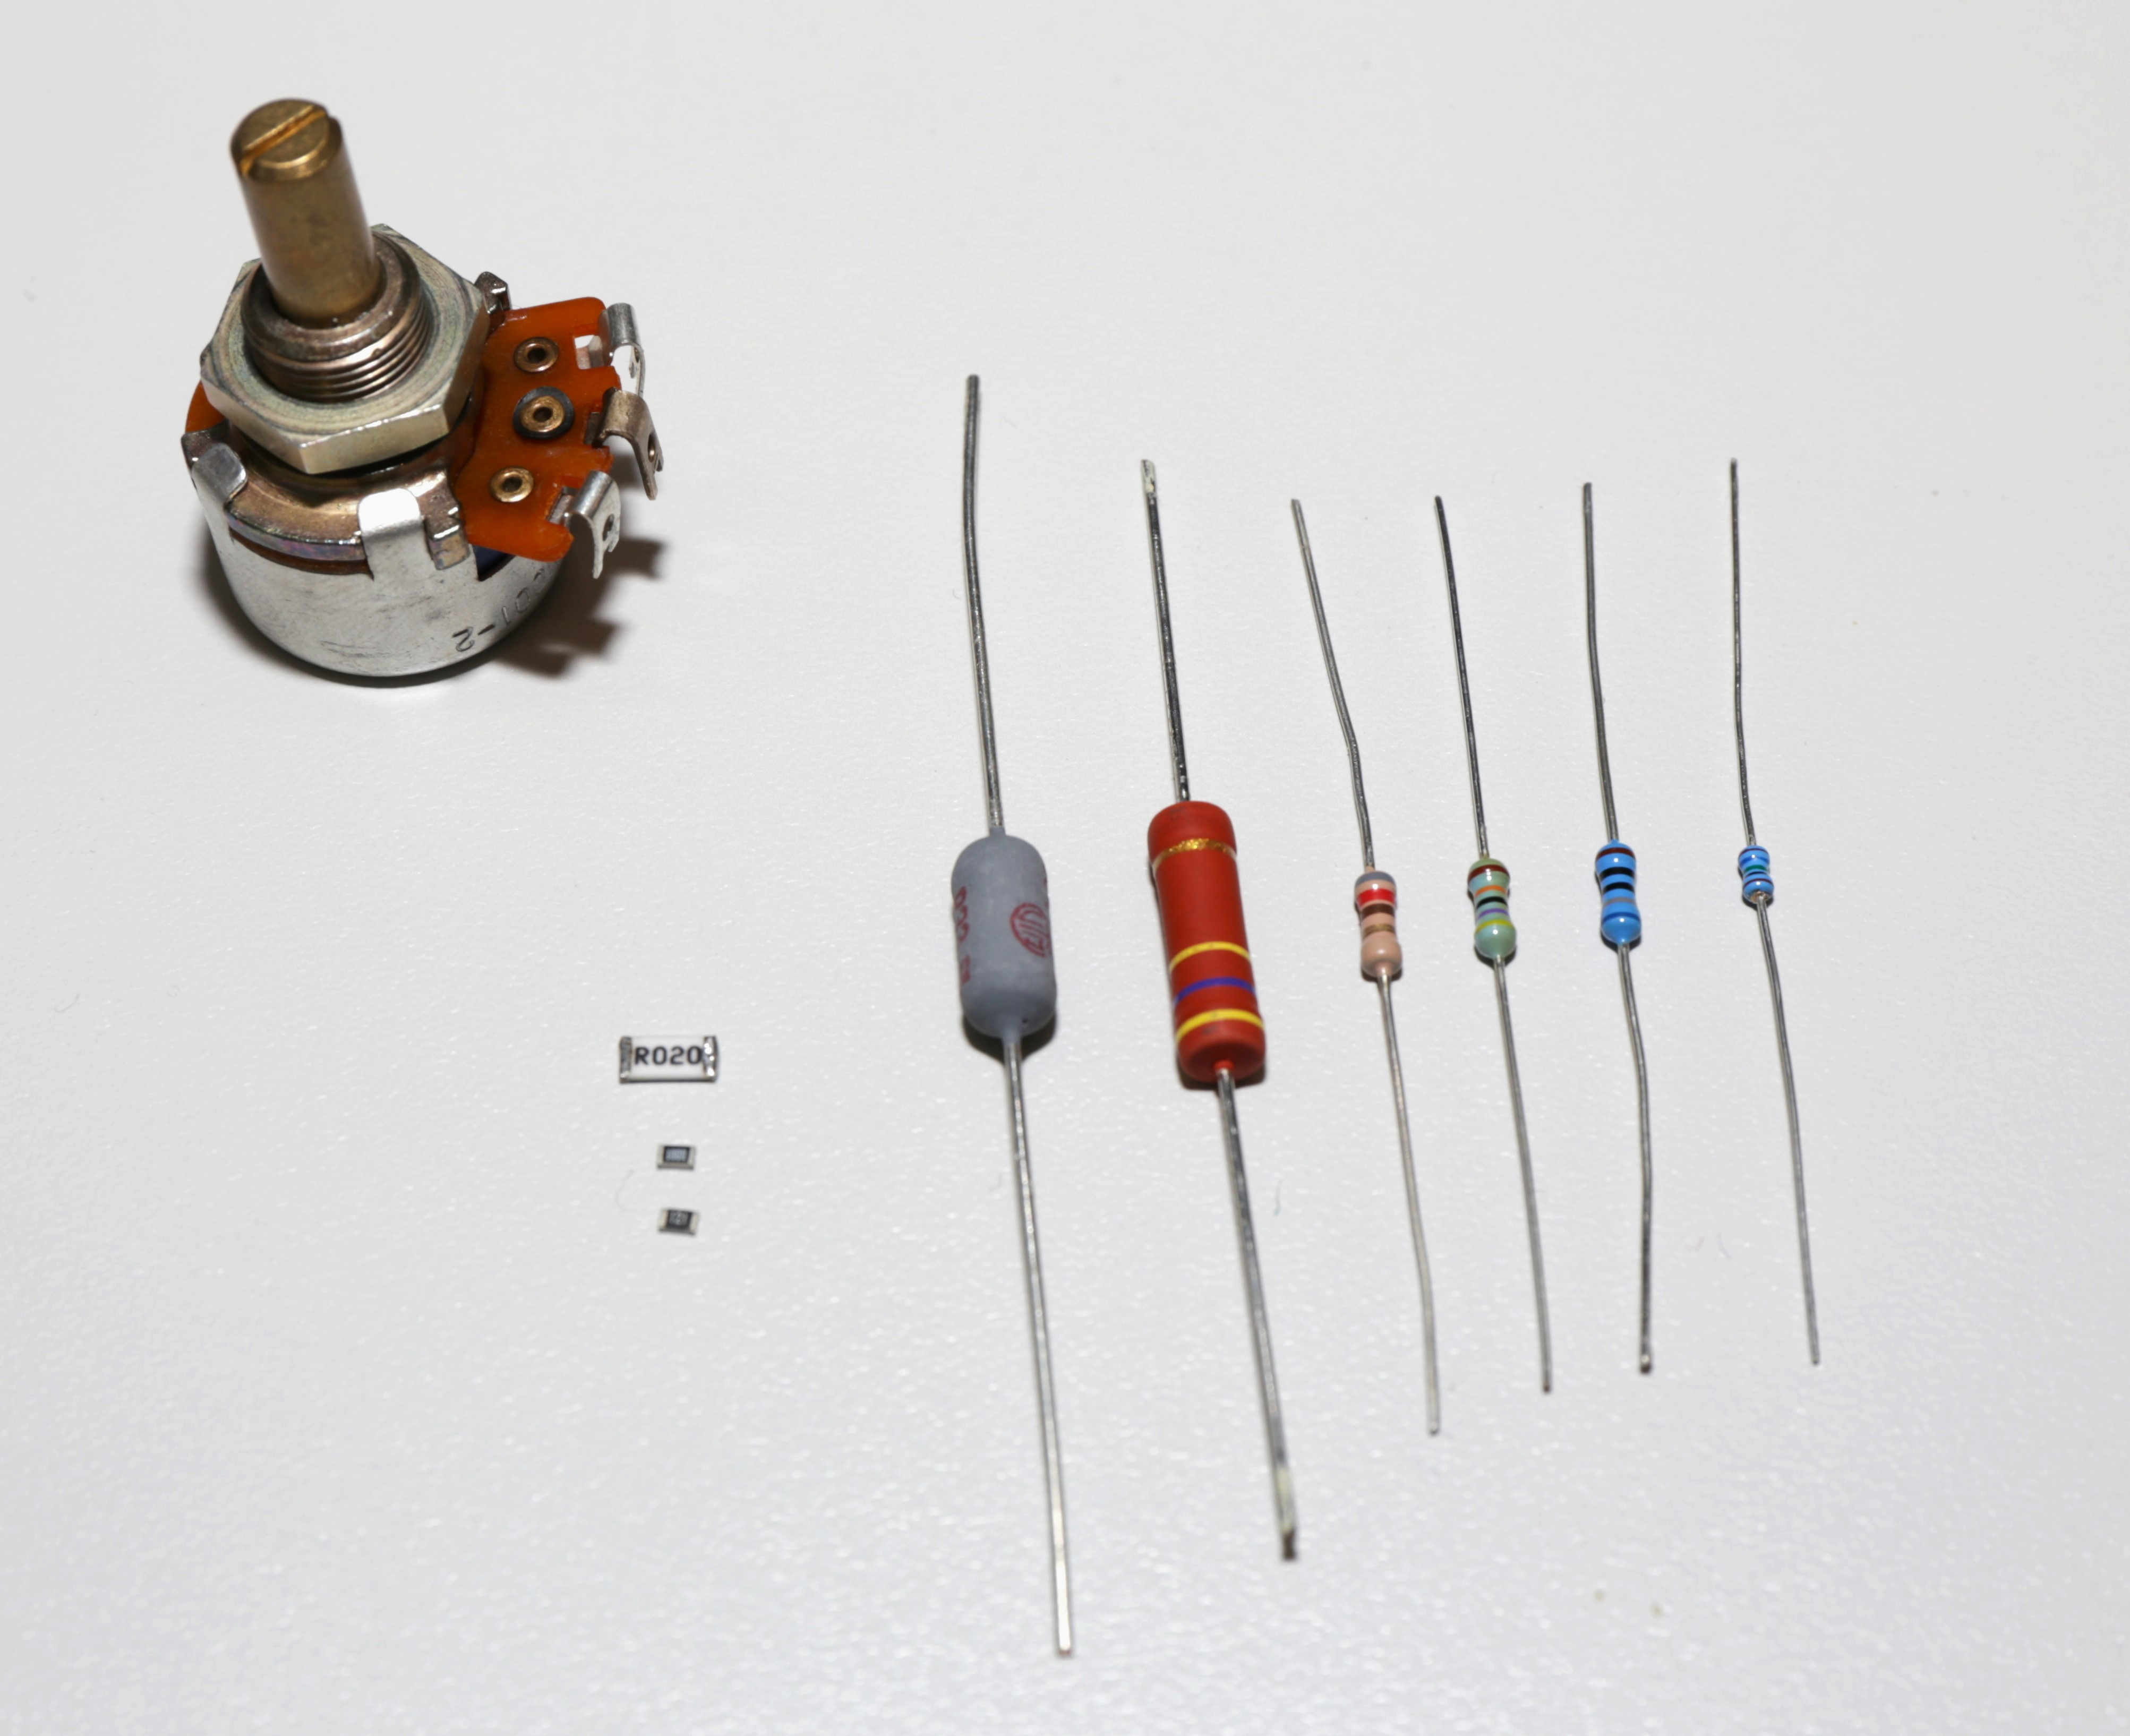
\includegraphics[width=0.5\textwidth]{wi}
		\caption{\textbf{Unterschiedliche ausführungen von Widerständen.} Darunter Drahtwiderstände, Potentiometer und SMD-Widerstände. Die Bauweise und das Material bestimmen die elektrischen Eigenschaften,
		 wie Widerstandswert, Belastbarkeit und Temperaturkoeffizient.}
		\label{fig:Widerstands Arten}}
	\end{figure}

	\speech{text}{1}{ % ToDo: für diesen speechtext muss diese Folie in ein begin(frame) eingebaut werden.
	Auf dem hier dargestellten Foto, das ist eigentlich noch ein Ausschnitt aus dem anfänglichen Foto, sehen Sie unterschiedliche Bauteilausführungen von Widerständen. 
Fangen wir erstmal mit dem Widerständen in der rechten Hälfte des Bildes an. Dort sehen Sie unterschiedliche Ausführungen eines sogenannten Feed-Through-Elements. 
Diese Bauelemente, da werden die Beinchen, die Drähte, die Anschlüsse geknickt und dann durch Bohrungen in der Platine durchgesteckt. 
Deshalb Feed-Through-Bauelement und dann an der Unterseite der Platine verlötet. 
Das heißt, der elektrische Kontakt dieses Bauelementes ist eigentlich genau auf der anderen Platinenseite wie das Bauelement selber. 
Das ist zum einen relativ aufwendig in der automatischen Bestickung und zum anderen hat das auch viele Nachteile, 
was parasitäre Effekte angeht für das Bauelement. Denn wir werden im späteren Verlauf sehen, dass die Zuleitung durch die Eigenschaften des Bauelementes deutlich beeinflusst. 
Deshalb werden heute sehr häufig die SMD-Widerstände eingesetzt. Das sind die ganz kleinen Chips, die Sie im linken unteren Teil sehen. 
Die gibt es in sehr unterschiedlichen Ausführungen, unterschiedlich groß, je nachdem für welches Raster Sie sich in Ihrer Platine entwickeln. 
SMD steht für Surface Mounted Device. Das heißt, diese Teile werden auf der Seite der Platine montiert und kontaktiert, wo auch die Leiterbahn ist. 
Das heißt, sie werden direkt auf die Leiterbahn gelötet und haben dadurch den Vorteil, dass sie weniger parasitäre Effekte zeigen. 
Nachteilig ist, dass sie meistens nicht die großen Leistungen aufnehmen können. 
Wenn man sich überlegt, das werden wir im späteren Verlauf sehen, dass die Leistung, die ein Widerstand aufnimmt, in Wärme gewandelt wird, 
ist irgendwie ersichtlich, dass zum Beispiel der zweite Widerstand von links, der rote, deutlich mehr Leistung aufnehmen kann als der kleine Chip ganz unten, 
schon alleine vom Volumen und der Masse. Oben links, das Bauteil, wo auch Mechanik-Elemente drin sind, das nennt man Potentiometer. 
Und das ist im Prinzip ein Widerstand mit einem festen Wert, aber sie haben einen sogenannten Mittelabgriff. 
Wenn wir an der rechten Seite des Baunelementes sehen oder schauen, dann sehen Sie dort drei Abgriffe. 
Und den vollen Widerstandswert, zum Beispiel 10 Kiloohm, den würden Sie erhalten, wenn Sie am oberen Kontakt und am unteren Kontakt kontaktieren. 
Und abhängig davon, wie Sie den Drehregler regeln, können Sie dann am Mittelabgriff den geteilten Widerstand abgreifen. 
Also zum Beispiel zwischen der mittleren Klemme und der oberen Klemme 7 Kiloohm und der mittleren Klemme und der unteren Klemme dann 3 Kiloohm, 
sodass in Summe wieder 10 Kiloohm vorhanden sind.
}

%%%%%%%%%%%%%%%%%%%%%%%%%%%%%%%%%%%%%%%%%%%%% Ende - Abbildung Widerstände %%%%%%%%%%%%%%%%%%%%%%%%%%%%%%%%%%%%

	
\s{
	In der Schaltungsentwicklung wird die physikalische Eigenschaft des ohm'schen Widerstandes genutzt, um die gewünschten Funktionen zu realisieren. 
	Die Abbildung \ref{fig:Widerstands Arten} zeigt verschiedene Ausführungen des Bauelements elektrischer Widerstand. Unabhängig von der Ausführung, 
	basieren alle ohm'schen Widerstände auf den grundlegenden Prinzipien der Physik, auf welche im Folgenden näher eingegangen wird.


%%%%%%%%%%%%%%%%%%%%%%%%%%%%%%%%%%%%%%%%%%%%% Anfang - Lernziele %%%%%%%%%%%%%%%%%%%%%%%%%%%%%%%%%%%%

\begin{Lernziele}{Leitfähigkeit und Widerstand} 
	Die Studierenden
	\begin{itemize}
	\item kennen das elektrische Bauelement Widerstand.
	\item können die unterschiedlichen Bauteilausführungen von Widerständen erklären.
	\item können anhand des spezifischen Widerstand $\rho$ oder des spezifischen Leitwertes $\kappa$ Berechnungen durchführen.
	\item können die Unterschiede in der Leitfähigkeit verschiedener Materialien basierend auf deren atomarer Struktur und Temperatur analysieren.
\end{itemize}
\end{Lernziele}
}


\end{frame}

%%%%%%%%%%%%%%%%%%%%%%%%%%%%%%%%%%%%%%%%%%%%% Ende - Lernziele %%%%%%%%%%%%%%%%%%%%%%%%%%%%%%%%%%%%
%%%%%%%%%%%%%%%%%%%%%%%%%%%%%%%%%%%%%%%%%%%%% Anfang - Leitfähigkeit %%%%%%%%%%%%%%%%%%%%%%%%%%%%%%%%%%%%

\subsection{Die elektrische Leitfähigkeit}
\begin{frame}[t]
	\ftx{Die elektrische Leitfähigkeit}
	
	Aus Modul 1 ist die Definition der Stromdichte $J$ und des Stromes $I$ bekannt.
	Durch Einsetzen der Formeln 2 und 3 in Formel 1 ergibt sich die Formel 4:
	\only<2->{
	\begin{equation}
		J=\frac{\Delta I}{\Delta A}
	\end{equation}}
	\only<3->{
	\begin{equation}
		I = \frac{\Delta Q}{\Delta t}
	\end{equation}}
	\only<4->{
	\begin{equation}
		\Delta V=\Delta A \cdot \Delta x \Leftrightarrow \Delta A = \frac{\Delta V}{\Delta x}
	\end{equation}}
	\only<5->{
	\begin{equation}
		J=\frac{\Delta Q \cdot \Delta x }{\Delta t \cdot \Delta V}
	\end{equation}}

			 \vspace{0.1cm}


\end{frame}

\subsection{Die elektrische Leitfähigkeit}
\begin{frame}[t]
	\ftx{Die elektrische Leitfähigkeit}

	Durch Einsetzen der aus Modul 1 bekannten Driftgeschwindigkeit $v_{el}$ und der Raumladungsdichte $\rho$ in die Formel 4,
	ergibt sich die Formel 7 für die Stromdichte.
	\only<2->{
	\begin{equation}
		v_{el}=\frac{\Delta x}{\Delta t}
	\end{equation}}
	\only<3->{
	\begin{equation}
		\rho = \frac{\Delta x}{\Delta V}
	\end{equation}}
	\only<4->{
	\begin{equation}
		\vec{J}=\rho \cdot \vec{v_{el}}
	\end{equation}}
	\only<5->{ \\
	Da die Geschwindigkeit immer einen Betrag und eine Richtung hat, ist die Stromdichte ebenfalls ein Vektor.
	}
			 \vspace{0.1cm}


\end{frame}


\subsection{Die elektrische Leitfähigkeit}
\begin{frame}[t]
	\ftx{Die elektrische Leitfähigkeit}

	Die Driftgeschwindigkeit $\vec{v_{el}}$ der freien Ladungsträger verhält sich proportional zum elektrischen Feld $\vec{E}$,
	jedoch in entgegengesetzter Richtung. Der Proportionalitätsfaktor wird auch als Elektronenbeweglichkeit $\mu_e$ bezeichnet.
	\only<2->{
	\begin{equation}
		\vec{v_{el}}=- \mu_e \cdot \vec{E}
	\end{equation}}
	\only<3->{ \\
	Die Raumladungsdichte $\rho$ setzt sich aus der Elementarladung $e^-$ und der Ladungsträgerdichte $n_e$, zusammen.
	Aufgrund der negativen Ladung von Elektronen, ergibt sich ein negatives Vorzeichen.
	}
	\only<4->{
	\begin{equation}
		\rho = - n_e \cdot e^-
	\end{equation}
	}
	\only<5->{ \\
Das Einsetzen von $\vec{v_{el}}$ und $\rho$ in die Formel 7 ergibt den folgenden Ausdruck:
	}
	\only<6->{
	\begin{equation}
		\vec{J} = (-n_e \cdot e^-) \cdot (-\mu_e \cdot \vec{E})
	\end{equation}
	}
			 \vspace{0.1cm}

\end{frame}



\subsection{Die elektrische Leitfähigkeit}
\begin{frame}[t]
	\ftx{Die elektrische Leitfähigkeit}
	Die Minuszeichen heben sich auf und es ergibt sich folgende Formel für die Stromdichte $\vec{J}$:
	\only<2->{
	\begin{equation}
		\vec{J}=n_e \cdot \mu_e \cdot e^- \vec{E}
	\end{equation}}
	\only<3->{ \\
	Die materialabhängigen Komponenten $n_e$ und $\mu_e$ sowie die Naturkonstante $e^-$ ergeben multipliziert die spezifische Leitfähigkeit $\kappa$:
	}\only<4->{
	\begin{equation}
		\kappa = n_e \cdot \mu_e \cdot e^-
	\end{equation}}
	\only<5->{ \\
	Zusammengefasst ergibt diese Darstellung die Beschreibung des ohmschen Gesetzes:
	\begin{equation}
		\vec{J}=\kappa \cdot \vec{E} \leftrightarrow \vec{E}=\frac{\vec{J}}{\kappa}
	\end{equation}
	}
			 \vspace{0.1cm}

\end{frame}

\begin{frame}[t]
	\ftx{Die elektrische Leitfähigkeit}

	\begin{equation}
		U_{12}=\int_{P_1}^{P_2} \vec{E} \mathrm{d}\vec{s}
	\end{equation}
	\only<2->{ \\
Da das elektrische Feld parallel zur Leitungslänge verläuft, ergibt sich das Skalarprodukt:
	}\only<3->{
\begin{equation}
	U_{12}=\int_{x=0}^{x=l} \vec{E} \mathrm{d}\vec{x}
\end{equation}}
\only<4->{ \\
Durch Einsetzen der umgestellten Formel 13 nach $\vec{E}$, folgt:
}\only<5->{
\begin{equation}
		U_{12}=\int_{0}^{l} \frac{J}{\kappa} \mathrm{d}x
	\end{equation}
}
			 \vspace{0.1cm}

\end{frame}

\begin{frame}[t]
	\ftx{Die elektrische Leitfähigkeit}
	
	Da es sich um ein homogenes Material handelt ist das $\kappa$ konstant.
	\only<2->{
\begin{equation}
		U_{12}=\frac{1}{\kappa}\cdot\int_{0}^{l} J \mathrm{d}x
	\end{equation}}
	\only<3->{ \\
			 
	Die folgende Formel für die Stromdichte $J$ ist aus Modul 1 bekannt:
	}\only<4->{
	\begin{equation}
		J=\frac{I}{A}
	\end{equation}
	}\only<5->{ \\
	Duch Einsetzen der Formel ergibt sich folgender Ausdruck:
	}\only<6->{
	\begin{equation}
		U_{12}=\frac{1}{\kappa}\cdot\int_{0}^{l} \frac{I}{A} \mathrm{d}x
	\end{equation}
	}
	\vspace{0.1cm}

\end{frame}

\b{
\begin{frame}[t]
	\ftx{Die elektrische Leitfähigkeit}
	Da die Querschnittsfläche $A$ ebenfalls konstant ist, kann das Integral aufgelöst werden:
	\only<2->{
	\begin{equation}
		U_{12}=\frac{1}{\kappa}\cdot \frac{I}{A} \cdot l
	\end{equation}}
	\only<3->{ \\
	Durch Umstellung ergibt sich:}
	\only<4->{
	\begin{equation}
		U_{12}=\frac{l}{A\cdot\kappa}\cdot I
	\end{equation}}
	\only<5->{ \\
	Da $\frac{l}{A\cdot\kappa}$ der elektrische Widerstand ist, ergibt sich folgende Vereinfachung:
	}
	\only<6->{
\begin{equation}
	U=R \cdot I
\end{equation}}

\end{frame}
}
\s{
	Die elektrische Leitfähigkeit sagt aus, wie gut ein Material Ladungsträger transportieren kann, also wie gut elektrischer Strom durch sie fließt.
	Sehr gut leitfähige Materialien werden Leiter (im Extremfall auch Supraleiter) genannt, während sehr schlecht leitende Materialien als Isolatoren bezeichnet werden.
	Zu den leitfähigen Medien zählen Metalle wie Kupfer, Silber, Aluminium und Gold, welche in der Elektrotechnik am häufigsten verwendet werden.
	Als Isolatoren werden zum Beispiel Kunststoffe (Polyethylen (PE), Polytetrafluorethylen (PTFE oder Teflon), Polyvinylchlorid (PVC) etc.), 
	speziell für die Anwendung als Isolator hergestellte Mineralöle, Silikone und Epoxidharz (z.B. als Vergussmasse) oder auch Papier verwendet.
	Des Weiteren gibt es Halbleiter wie Silizium und Germanium, deren Leitfähigkeit zwischen denen von Leitern und Isolatoren einzuordnen sind.
	Ihre Leitfähigkeit kann durch Dotierung und äußere Einflüsse wie Temperatur und Licht verändert werden.
	Diese Eigenschaften werden bei Bauteilen wie Dioden oder Transistoren genutzt, um bestimmte Funktionen zu realisieren. 
	Die verschiedenen Arten und Eigenschaften von Halbleiter sind sehr umfangreich und werden in späteren Modulen behandelt.
	Vollständigkeitshalber sei noch erwähnt, dass flüssige Medien wie Säuren oder Salzlösungen leitfähig sind und als Elektrolyt bezeichnet werden.
	Außerdem gibt es auch ionisierte Gase, die frei bewegliche Ladungsträger enthalten und elektrische Ströme leiten können. 
	Diese leitfähigen Gase werden Plasmen genannt, welche in diesem Modul ebenfalls nicht behandelt werden.
}

\subsection{Driftverhalten von Elektronen in Leitern}
\begin{frame}
	\ftx{Driftverhalten von Elektronen in Leitern}


% Wieso kommt es zu unterschiedlichen Widerstandswerten? Was ist die Driftgeschwindigkeit? Anstoßen gegen Atomrümpfe
\s{
	In Modul 1 wurde bereits vermittelt, dass der elektrische Stromfluss die gerichtete Bewegung von freien Ladungsträgern ist.
	Im Fall eines Leiters sind dies die negativen Ladungsträger, also die Elektronen, welche sich frei im Material bewegen können.
	Die Struktur eines solchen Materials besteht aus einem festen Gitter von Atomrümpfen und frei beweglichen Elektronen.
	Sowohl die Beweglichkeit der Elektronen $\mu_{\mathrm{e}}$, als deren Anzahl, ist materialabhängig.
	Im feldfreien Raum bewegen sich diese Elektronen zufällig in alle Richtungen, was zu einem neutralen Zustand führt.
	Da es sich hierbei um keine gerichtete sondern um eine in alle Richtungen gleichverteilte Bewegung handelt, ist kein Stromfluss feststellbar. 
	Dennoch führt diese ungerichtet, von der Temperatur abhängige, Bewegung der Ladungsträger zu elektrotechnischen Effekten: 
	In empfindlichen Schaltungen wird sie als Rauschen wahrgenommen. Die freien Ladungsträger sind sehr viel leichter als die im Gitter verankerten Atomrümpfe, 
	so dass es bei einem Aufprall eines in Bewegung befindlichen Elektrons auf einen Atomrumpf zu einem unelastischen Stoss kommt und sich die Bewegungsrichtung des Elektrons ändert.
	Dieses Verhalten ist in Abbildung \ref{fig:Elektronenbewegung} zu sehen.
}

% % Nachdem das grundlegende Verständnis von Widerständen erklärt wurde, kann das Thema auch auf atomarer Ebene behandelt werden. Diese Betrachtungsweise ist wichtig, um die mathematischen Zusammenhänge besser nachvollziehen zu können 
% % und das sonst schwer greifbare Thema der Elektrizität etwas zu veranschaulichen.
% % Der atomare Aufbau eines Materials erlaubt es den Elektronen sich in der Struktur frei zu bewegen. Im neutralen zustand ohne anlegen einer Spannung bewegen sich die Elektronen in alle Richtungen. 
% % Da die Wahrscheinlichkeit der Bewegungsrichtung gleichverteilt ist, ergibt sich der Mittelwert 0, wodurch kein elektrischer Strom im Leiter fließt.
% % Die nachfolgende Grafik zeit die Bewegung der Elektronen in einer atomaren Struktur.
% % Sobald nun eine Spannung an den Leiter angelegt wird, entsteht ein elektrisches Feld, wodurch sich die Bewegungsrichtung der Elektronen ausrichtet. Die Beweglichkeit und die Anzahl freier Elektronen können in der spezifischen Leitfähigkeit Kappa zusammengefasst. 
% % Die Anzahl der freien Ladungsträger hängt vom Material ab. Die Beweglichkeit wiederum hängt von der Temperatur ab. Die theoretisch niedrigste Temperatur beträgt 0 Kelvin. Bei diesem absoluten Nullpunkt bewegen sich die freien Elektronen nicht mehr frei im Raum, 
% % sodass sie sich nur dem elektrischen Feld ausrichten können. Dabei wird der kleinste materialspezifische Widerstandswert erreicht. Bei bestimmten Materialien ist so auch die realisierung eines Supraleiters möglich, welche ihren elektrischen Widerstand verlieren.
% % Die Beweglichkeit und die Anzahl freier Elektronen können in der spezifischen Leitfähigkeit Kappa zusammengefasst. Die folgende Formel beschreibt das Ohmsche gesetz in vektorieller Art.
% % Die bisherige Definition des Begriffs Widerstand beschreibt den (Rho) materialspezifischen Widerstandswert eines Bauteils. 

%%%%%%%%%%%%%%%%%%%%%%%%%%%%%%%%%%%%%%%%%%%%% Anfang - Grafik Elektronenbewegung ungerichtet %%%%%%%%%%%%%%%%%%%%%%%%%%%%%%%%%%%%
\b{
		\begin{itemize}
		\item Ungerichte Bewegung freier Elektronen (blau) zwischen positiv geladenen Atomrümpfen (rot)
	    \end{itemize}
}


\begin{figure}[H]
	\centering
	\includesvg[width=0.8\textwidth]{Elektronenbewegung}
	\s{\caption{\textbf{Ungerichtete Bewegung freier Elektronen.} Zeigt die freien Elektronen (blau) zwischen positiv geladenen Atomrümpfen (rot). Solche Bewegungen sind charakteristisch für Metalle im Ruhezustand,
	 wo die Elektronen sich zufällig bewegen, ohne eine bevorzugte Richtung, solange kein äußeres elektrisches Feld anliegt.}}
	\label{fig:Elektronenbewegung}
\end{figure}

\end{frame}
%%%%%%%%%%%%%%%%%%%%%%%%%%%%%%%%%%%%%%%%%%%%% Ende - Grafik Elektronenbewegung ungerichtet %%%%%%%%%%%%%%%%%%%%%%%%%%%%%%%%%%%%
%%%%%%%%%%%%%%%%%%%%%%%%%%%%%%%%%%%%%%%%%%%%% Anfang - Driftverhalten %%%%%%%%%%%%%%%%%%%%%%%%%%%%%%%%%%%%
\s{
Sobald sich ein Leiter in einem elektrischen Feld befindet, wirkt auf die Elektronen die Coulomb-Kraft, 
so dass sich ihre zufällige Bewegungsrichtung in eine gerichtete Bewegung ändert, welche entgegengesetzt zur Feldrichtung zeigt (Abb.\ref{fig:Elektronenbewegung gerichtet}). 
Diese gerichtete Bewegung der Ladungsträger wird als Stromfluss bezeichnet (vgl. Modul 1).
Allerdings kommt es auch weiterhin zu Stößen mit den Atomrümpfen. Diese führen letztlich zu einer Abschwächung der gerichteten Bewegung und somit des Stroms (vgl. Abb.\ref{fig:Elektronenbewegung gerichtet}). 
Da sich die Atomrümpfe mit steigender Temperatur stärker bewegen, nimmt die Stoßwahrscheinlichkeit der Elektronen bei steigender Temperatur zu.
\\
}

%%%%%%%%%%%%%%%%%%%%%%%%%%%%%%%%%%%%%%%%%%%%% Anfang - Grafik Elektronenbewegung gerichtet %%%%%%%%%%%%%%%%%%%%%%%%%%%%%%%%%%%%

\begin{frame}
	
		\ftx{Driftverhalten von Elektronen in Leitern}

	\b{
		\begin{itemize}
		\item Gerichtete Bewegung von Elektronen entgegen der Richtung des elektischen Feldes $\vec{E}$
	    \end{itemize}

		\begin{figure}[H]
			\centering
			\includesvg[width=0.8\textwidth]{Elektronenbewegung_gerichtet}
		\end{figure}
	}
\end{frame}
\s{
\begin{figure}[H]
	\centering
	\includesvg[width=0.8\textwidth]{Elektronenbewegung_gerichtet}
	\caption{\textbf{Gerichtete Bewegung von Elektronen.} Unter Einfluss eines elektrischen Feldes $\vec{E}$ bewegen sich die freien Elektronen in einem
	Leiter entgegen der Feldrichtung, was den elektrischen Stromfluss $I$ erklärt.}
	\label{fig:Elektronenbewegung gerichtet}
\end{figure}
}



%%%%%%%%%%%%%%%%%%%%%%%%%%%%%%%%%%%%%%%%%%%%% Ende - Grafik Elektronenbewegung gerichtet %%%%%%%%%%%%%%%%%%%%%%%%%%%%%%%%%%%%

\s{
Dieses Verhalten der Elektronen wird auch Driftverhalten genannt, welches stark vom Material anhängt.
Da die atomare Zusammensetzung materialabhängig ist, unterscheidet sich auch die Anzahl der freien Elektronen, sowie deren Beweglichkeit $\mu_{\mathrm{e}}$.
Diese beiden Eigenschaften werden unter dem Begriff der spezifischen Leitfähigkeit $\kappa$ zusammengefasst. 
Mit der spezifischen Leitfähigkeit kann somit die Driftgeschwindigkeit der Elektronen in der Gitterstruktur des Leiters ermittelt werden.
Der folgende Abschnitt befasst sich mit eben diesen Eigenschaften.
}

%%%%%%%%%%%%%%%%%%%%%%%%%%%%%%%%%%%%%%%%%%%%% Ende - Driftverhalten %%%%%%%%%%%%%%%%%%%%%%%%%%%%%%%%%%%%

%%%%%%%%%%%%%%%%%%%%%%%%%%%%%%%%%%%%%%%%%%%%% Anfang - Mathematik / Berechnung Widerstand %%%%%%%%%%%%%%%%%%%%%%%%%%%%%%%%%%%%
\begin{frame}
	\ftx{Mathematische Zusammenhänge der Leitfähigkeit}
\subsection{Mathematische Zusammenhänge der Leitfähigkeit}
\b{

\begin{equation*}
[\kappa] = 1\,\, \frac{\text{Siemens}}{\text{meter}} = 1\,\, \frac{\text{S}}{\text{m}} = 1\,\,\frac{\text{1}}{\Omega \cdot \text{m}}
	 \end{equation*}
	 \vspace{0.1cm}
\begin{equation*}
	\kappa = \frac{1}{\rho_\mathrm{R}}
\end{equation*}

\begin{equation*}
	\rho_\mathrm{R} = \rho_\mathrm{{20^\circ C}} \cdot (1 + \alpha (\vartheta - 20\mathrm{^\circ C}))
\end{equation*}
}% nur Folien
\s{
Die unterschiedlichen atomaren Zusammensetzungen der Materialien führen zu einer materialabhängigen, elektrischen Leitfähigkeit.
Die materialspezifische Eigenschaft bestehen aus der spezifischen Leitfähigkeit $\kappa$ (Kappa), bzw. dem spezifischen Widerstand $\rho_\mathrm{R}$ (rho) 
welche antiproportional zueinander stehen, sowie dem jeweiligen Temperaturkoeffizient $\alpha$, welcher sich je nach Material unterscheidet.



%%%%%%%%%%%%%%%%%%%%%%%%%%%%%%%%%%%%%%%%%%%%% Anfang - Formeln %%%%%%%%%%%%%%%%%%%%%%%%%%%%%%%%%%%%
 \begin{equation*}
[\kappa] = 1\,\, \frac{\text{Siemens}}{\text{m}} = 1\,\, \frac{\text{S}}{\text{m}} =  1\,\, \frac{\text{1}}{\Omega \cdot \text{m}}
 \end{equation*}
 \vspace{0.1cm}
\begin{equation}
	\kappa = \frac{1}{\rho_\mathrm{R}} 
\end{equation}

%%%%%%%%%%%%%%%%%%%%%%%%%%%%%%%%%%%%%%%%%%%%% Ende - Formeln %%%%%%%%%%%%%%%%%%%%%%%%%%%%%%%%%%%%
% \s{
% Zur Berechnung des Widerstandwertes bei einer konkreten Temperatur, wird die Temperaturdifferenz zu $20^\circ C$ gebildet und dieser Wert mit dem Temperaturkoeffizienten multipliziert.
% Dieser Wert wird mit dem bekannten Referenzwert bei $20^\circ C$ multipliziert und mit diesem addiert.
% }
%%%%%%%%%%%%%%%%%%%%%%%%%%%%%%%%%%%%%%%%%%%%% Anfang - 	Formeln Kappa, Roh	  %%%%%%%%%%%%%%%%%%%%%%%%%%%%%%%%%%%%

\begin{equation}
	\rho_\mathrm{R} = \rho_\mathrm{{20^\circ C}} \cdot (1 + \alpha (\vartheta - 20\mathrm{^\circ C}))
	\end{equation}
}% nur im Skript
%%%%%%%%%%%%%%%%%%%%%%%%%%%%%%%%%%%%%%%%%%%%% Ende 	- 	Formeln Kappa, Roh	  %%%%%%%%%%%%%%%%%%%%%%%%%%%%%%%%%%%%
\s{
Für $\vartheta$ (Theta) wird die Temperatur des Leiters eingetragen. Daraus ergibt sich durch ($\vartheta - 20\mathrm{^\circ C}$) die Temperaturdifferenz des Leiters zwischen der vorhandenen Temperatur des Leiters und den $\mathrm{20^\circ C}$, bei welchen der Referenzwert ermittelt wurde.
Werden $20\mathrm{^\circ C}$ für $\vartheta$ (Theta) eingesetzt, fällt auch das $\alpha$ weg und es bleibt der Referenzwert $\rho_\mathrm{20\mathrm{^\circ C}}$ übrig. 
In der folgenden Tabelle sind beispielhaft einige Materialien mit deren spezifischen Eigenschaften dargestellt:
}
\end{frame}
%%%%%%%%%%%%%%%%%%%%%%%%%%%%%%%%%%%%%%%%%%%%%%%%% Anfang - Tabelle Eigenschaften %%%%%%%%%%%%%%%%%%%%%%%%%%%%%%%%%%%%%%%%%%
%%%
%%%	In der Tabelle fehlen die Referenzwerte bei 20°C, sonst kann Formel 1.2 nicht angewendet werden.
%%%
%%%%%% Einfache Tabelle
\begin{frame}
	\ftx{Spezifische Leitfähigkeiten und Temperaturkoeffizienten}
	\begin{table}[H]
		\centering
		\resizebox{0.8\textwidth}{!}{%
		\begin{tabular}{@{}l c c@{}}
		\toprule
		\textbf{Material} & {\textbf{Spezifische Leitfähigkeit} [$\kappa$] = S/m} & 
		{\textbf{Temperaturkoeffizient} [$\alpha$] = 1/K} \\
		\midrule
		Silber & $6.1\cdot 10^{7}$ & 0.0038 \\
		Kupfer & $5.8 \cdot 10^{7}$ & 0.0038 \\
		Gold & $4.5 \cdot 10^{7}$ & 0.0034 \\
		Aluminium & $3.7 \cdot 10^{7}$ & 0.004 \\
		Eisen & $1.0 \cdot 10^{7}$ & 0.0065 \\
		Graphit & $3 \cdot 10^{6}$ & -0.0002  \\
		Silizium (dotiert) & {$1 - 10^6$} & -0.075 \\
		Leitungswasser & $5.0 \cdot 10^{-3}$ & {-} \\
		Luft & $4.0 \cdot 10^{-15}$ & {-} \\
		\bottomrule
		\end{tabular}%
		}
		\s{\caption{\textbf{Spezifische Leitfähigkeiten und Temperaturkoeffizienten verschiedener Materialien.} Metalle wie Silber und Kupfer haben hohe Leitfähigkeiten, 
		während isolierende Materialien wie Luft eine sehr geringe Leitfähigkeit besitzen.}}
		\label{tab:specific_resistance}
		\end{table}
\end{frame}

%%%%%%%%%%%%%%%%%%%%%%%%%%%%%%%%%%%%%%%%%%%%%%%%% Ende - Tabelle Eigenschaften %%%%%%%%%%%%%%%%%%%%%%%%%%%%%%%%%%%%%%%%%%
\begin{frame}
	\ftx{Der Leitwert}

\b{
	\begin{equation*}
	[G] = 1\, \text{Siemens} = 1\, \text{S} = 1\,\, \frac{\text{1}}{\Omega}
	\end{equation*}
	\vspace{0.1cm}
	\begin{equation*}
		G = \frac{1}{R}
	\end{equation*}
}

\end{frame}
\s{
Äquivalent zur spezifischen Leitfähigkeit $\kappa$ und zum spezifischen Widerstand $\rho_\mathrm{R}$,
kann der entsprechende Widerstand $R$, bzw. Leitwert $G$ eines Körpers bestimmt werden.

%%%%%%%%%%%%%%%%%%%%%%%%%%%%%%%%%%%%%%%%%%%%%%%%% Anfang - G = 1/R %%%%%%%%%%%%%%%%%%%%%%%%%%%%%%%%%%%%%%%%%%
\begin{equation*}
	[G] = 1\, \text{Siemens} = 1\, \text{S} = 1\,\, \frac{\text{1}}{\Omega}
	 \end{equation*}
	 \vspace{0.1cm}
\begin{equation}
	G = \frac{1}{R} 
\end{equation}
%%%%%%%%%%%%%%%%%%%%%%%%%%%%%%%%%%%%%%%%%%%%%%%%% Ende - G = 1/R %%%%%%%%%%%%%%%%%%%%%%%%%%%%%%%%%%%%%%%%%%

Der Wert der elektrischen Leitfähigkeit bzw. des Widerstandes eines Leiters, ergibt sich darüber hinaus aus den geometrischen Eigenschaften.
Sowohl die Länge $l$ als auch die Querschnittsfläche $A$ tragen zum Leitwert bzw. Widerstandswert bei.
Abbildung \ref{fig:Widerstand} zeigt einen solchen Leiter mit seinen Eigenschaften.
}

%%%%%%%%%%%%%%%%%%%%%%%%%%%%%%%%%%%%%%%%%%%%% Anfang - Abbildung Leiter %%%%%%%%%%%%%%%%%%%%%%%%%%%%%%%%%%%%

\begin{frame}
	\ftx{Geometrische Eigenschaften}
	
	\begin{figure}[H]
			\centering
			   \b{ 
				\begin{itemize}
				\item Länge $l$
				\item Querschnittsfläche $A$
				\item Spezifische Leitfähigkeit $\kappa$
				\end{itemize}
				\includesvg[width=0.9\textwidth]{Widerstand}}
			   \s{\includesvg[width=0.8\textwidth]{Widerstand}
			   \caption{\textbf{Geometrische Darstellung eines Widerstands.} Das elektrische Feld \(\vec{E}\) erzeugt eine Stromdichte 
			   \(\vec{J}\) durch den Widerstand. Die Beziehung zwischen der Stromdichte und dem elektrischen Feld wird durch das Ohmsche Gesetz
			    \( \vec{J} = \kappa \cdot \vec{E} \) beschrieben.}}
	   
			   \label{fig:Widerstand}
	\end{figure}

%%%%%%%%%%%%%%%%%%%%%%%%%%%%%%%%%%%%%%%%%%%%% Ende - Abbildung Leiter %%%%%%%%%%%%%%%%%%%%%%%%%%%%%%%%%%%%
\s{
Die Stromdichte $\vec{J}$ ergibt sich dabei aus dem elektrischen Feld $\vec{E}$ und der spezifischen Leitfähigkeit $\kappa$.
Die Stromdichte ist dabei geometrieunabhängig. Erst zur Berechnung des Stromes $I$ müssen die Länge und die Querschnittsfläche mit einbezogen werden.
Mit der folgenden Formel lässt sich der Widerstandswert berechnen:
}
\end{frame}
%%%%%%%%%%%%%%%%%%%%%%%%%%%%%%%%%%%%%%%%%%%%% Anfang - 	Formeln R		  %%%%%%%%%%%%%%%%%%%%%%%%%%%%%%%%%%%%
\begin{frame}
	\ftx{Geometrische Eigenschaften}
	\b{
		
		\begin{itemize}
		\item Allgemeine Formel für den Widerstand in Bezug auf die Materialeigenschaften
	    \end{itemize}
		\vspace{1cm}
		\begin{equation*}
			[R] = 1\, \text{Ohm} = 1\, \text{$\Omega$}
		\end{equation*}
		\vspace{0.1cm}
		\begin{equation*}
			R = \rho_\mathrm{R} \cdot \frac{l}{A} 
		\end{equation*}
		\begin{align*}
			\rho_\mathrm{R} &: \text{spezifischer Widerstand des Materials } (\Omega \text{m}) \\
			l &: \text{Länge des Materials (m)} \\
			A &: \text{Querschnittsfläche des Materials } (\text{m}^2) \\
		\end{align*}

	}
\end{frame}
\s{
	\begin{equation*}
		[R] = 1\, \text{Ohm} = 1\, \text{$\Omega$}
	\end{equation*}
	\vspace{0.1cm}
\begin{equation}
	R = \rho_\mathrm{R} \cdot \frac{l}{A}   
\end{equation}

\begin{align*}
	\rho_\mathrm{R} &: \text{spezifischer Widerstand des Materials } (\Omega \text{m}) \\
	l &: \text{Länge des Materials (m)} \\
	A &: \text{Querschnittsfläche des Materials } (\text{m}^2) \\
\end{align*}
}

%%%%%%%%%%%%%%%%%%%%%%%%%%%%%%%%%%%%%%%%%%%%% Ende 	- 	Formeln R			  %%%%%%%%%%%%%%%%%%%%%%%%%%%%%%%%%%%%
\s{
\textbf{Einführung in die Darstellung von Schaltkreisen}


In der Elektrotechnik werden zur Darstellung von elektrischen Netzwerken sogenannte Schaltbilder verwendet.
Inhalt dieser Schaltbilder sind Schaltsymbole, welche für die elektrischen Eigenschaften bzw. ganze Bauelemente, verwendet werden.
Abbildung \ref{fig:erstes_schaltbild} zeigt beispielhaft ein solches Schaltbild.
}
\begin{frame}
	\ftx{Einführung in die Darstellung von Schaltkreisen}
\begin{figure}[H]
	\centering
\hspace{1cm} % Um es in der Mitte zu haben
	\begin{circuitikz}
  \draw (0,3) to[V, i, name=I] (0,0)
		(0,3) -- (1.5,3)
		(1.5,3) to[switch, l={Schalter}] (2.5,3)
		(2.5,3) -- (4,3)
		(4,3) to[lamp, l={Glühlampe}] (4,0);
      	\draw (3,0) to [R, l={Widerstand}] (1,0);
		\draw (0,0) -- (1,0);
		\draw (3,0) -- (4,0);		            
		
		% Draw current arrow
		\iarrmore{I}{$I$};

		% Draw voltage arrows
		\draw[-latex, thick, draw=voltage] (-0.6,2)  to node[midway,left,  color=voltage] {$U_\mathrm{q}$} (-0.6,1);
		
	\end{circuitikz}
	\s{\caption{\textbf{Schaltplan einer Reihenschaltung.} Die aus einer Gleichspannungsquelle einem Schalter, einem Verbraucher und einem Widerstand besteht.}}
	\label{fig:erstes_schaltbild}
\end{figure}
\end{frame}
\s{
Das Schaltbild besteht aus vier Elementen, welche mit Linien verbunden sind. Es stellt eine Reihenschaltung bestehend aus
einer Spannungsquelle, einem Schalter, einer Glühlampe und einem Widerstand, dar. Der Widerstand stellt den Leitungswiderstand der gesamten Leitung dar,
während die Verbindungslinien per Definition ideale Verbindungen ohne weitere Eigenschaften darstellen.

Des Weiteren ist eine Spannung $U_{\mathrm{q}}$, sowie der Strom $I$ eingezeichnet, welcher jedoch erst fließen kann, wenn der Schalter geschlossen wird.
Im Folgenden werden die drei grundlegenden elektrischen Eigenschaften, sowie deren Schaltsymbole tiefer behandelt.
}
%%%%%%%%%%%%%%%%%%%%%%%%%%%%%%%%%%%%%%%%%%%%% Anfang - Widerstand als Bauelement %%%%%%%%%%%%%%%%%%%%%%%%%%%%%%%%%%%%
\begin{frame}
	\ftx{Widerstand als Bauelement}
\subsection{Widerstand als Bauelement}

\s{
Mit Hilfe der im vorherigen Abschnitt kennengelernten Methode zu Berechnung des Widerstandes, 
kann der Widerstandswert elektrischer Leitungen, oder auch anderer leitender Objekte, ermittelt werden.
Sobald ein Widerstandswert bekannt ist, wird dieser in elektrischen Schaltbildern einem Schaltsymbol zugeordnet.
So können verschiedene Komponenten und deren Eigenschaften miteinander verbunden werden, um deren Verhalten zu ermitteln.
Abbildung \ref{fig:resistor-symbols_} zeigt zwei gängige Schaltzeichen für den Widerstand.
}% nur im Skript

%%%%%%%%%%%%%%%%%%%%%%%%%%%%%%%%%%%%%%%%%%%%%% Anfang - Widerstand EU und US %%%%%%%%%%%%%%%%%%%%%%%%%%%%%
% Europäisches und amerikanisches Symbol
\b{
		\begin{itemize}
		\item Europäisches (links) und amerikanisches (rechts) Schaltelement für Widerstand
	    \end{itemize}
\begin{figure}[H]
    \centering
    \begin{circuitikz}
        % Europäisches Symbol
		\draw (0,0) to [R,i,v, name=R, o-, l=$R$] (2.5,0)
		to [short,-o] (2.5,0);
        
        % Amerikanisches Symbol
		\draw (6,0) to [R,i,v, name=R, o-, l=$R$, american] (8.5,0)
		to [short,-o] (8.5,0);

    \end{circuitikz}
\end{figure}

}% nur Folie
\s{
\begin{figure}[H]
    \centering
    \begin{circuitikz}
        % Europäisches Symbol
		\draw (0,0) to [R,i,v, name=R, o-, l=$R$] (2.5,0)
		to [short,-o] (2.5,0);
        
        % Amerikanisches Symbol
		\draw (6,0) to [R,i,v, name=R, o-, l=$R$, american] (8.5,0)
		to [short,-o] (8.5,0);

    \end{circuitikz}
    \caption{\textbf{Schaltungselement für Widerstand.} Europäisches (links) und amerikanisches (rechts).}
    \label{fig:resistor-symbols_}
\end{figure}
}

%%%%%%%%%%%%%%%%%%%%%%%%%%%%%%%%%%%%%%%%%%%%%% Ende - Widerstand EU und US 	  %%%%%%%%%%%%%%%%%%%%%%%%%%%%%

\s{
	Sobald eine Gleichspannungsquelle an einen Widerstand $R$ angeschlossen wird, verhalten sich Strome und Spannungen linear.
	Abbildung \ref{fig:idealer Widerstand} zeigt den durch den Widerstand fließenden Strom $I_\mathrm{R}$, 
	sowie die abfallende Spannung $U_\mathrm{R}$.
}

%%%%%%%%%%%%%%%%%%%%%%%%%%%%%%%%%%%%%%%%%%%%%% Anfang - Widerstand Schaltbild %%%%%%%%%%%%%%%%%%%%%%%%%%%%%
%%%%% Ideal und reeller Widerstand
\b{
	\begin{itemize}
		\item Der idealer Widerstand als Schaltsymbol 
	    \end{itemize}
% Idealer Widerstand
\begin{figure}[H]
	\centering
	\begin{circuitikz}
		% Idealer Widerstand
		\draw (0,0) to [R,i,v, name=R, o-, l=$R$] (2.5,0)
					to [short,-o] (2.5,0);
		\iarrmore{R}{$I_\mathrm{R}$};
		\varrmore{R}{$U_\mathrm{R}$};

	\end{circuitikz}
\end{figure}
}
\end{frame}
\s{
	% Idealer Widerstand
	\begin{figure}[H]
		\centering
		\begin{circuitikz}
			% Idealer Widerstand
			\draw (0,0) to [R,i,v, name=R, o-, l=$R$] (2.5,0)
						to [short,-o] (2.5,0);
			\iarrmore{R}{$I_\mathrm{R}$};
			\varrmore{R}{$U_\mathrm{R}$};
	
		\end{circuitikz}
		\caption{\textbf{Idealer Widerstand.} Zeigt den Spannungsabfall über den Widerstand und den Stromfluss durch ihn.}
		\label{fig:idealer Widerstand}
	\end{figure}
}

	%%%%%%%%%%%%%%%%%%%%%%%%%%%%%%%%%%%%%%%%%%%%%% Ende - Widerstand Schaltbild %%%%%%%%%%%%%%%%%%%%%%%%%%%%%
	\begin{frame}
		\ftx{Widerstand als Bauelement}
	\s{
		Das Schaltsymbol des Widerstandes wird in Schaltungen immer als idealer Widerstand berücksichtigt. 
		Unter Vernachlässigung der Temperaturabhängigkeit trifft dies im Gleichspannungsfall auch weitestgehend zu (Schaltvorgänge ausgenommen).
		In der Realität gibt es viele Situationen, in denen ein realer Widerstand kein lineares Verhalten aufweisen kann.
		Verschiedene Quellenarten werden im Abschnitte 1.2 zu Spannungs- und Stromquellen behandelt.
		Zum Verständnis der Abbildung \ref{fig:ESB realen Widerstand} ist es ratsam, zuvor die Abschnitte 1.3 und 1.4 gelesen zu haben.
	}
	%%%%%%%%%%%%%%%%%%%%%%%%%%%%%%%%%%%%%%%%%%%%%% Anfang - realer Widerstand Schaltbild %%%%%%%%%%%%%%%%%%%%%%%%%%%%%
\b{
	\begin{itemize}
		\item Ersatzschaltbild eines realen Widerstands mit $C_\mathrm{p}$ und $L_\mathrm{s}$
	    \end{itemize}
}
	% Realler Widerstand
\begin{figure}[H]
    \centering
    \begin{circuitikz}
        \draw (-0.5,0.75) to [short, o-] (0,0.75);
        \draw (1.6,0) to [C,i,v, name=C, l={$C_\mathrm{p}$}] (4,0)
        (3.8,0)--(5.6,0)
		(0,0)--(2,0);
        \draw (0,0) to [short] (0,1.5);
		\draw (5.6,0) to [short] (5.6,1.5);
        \draw (0,1.5)
              to [L,i,v, name=L, l={$L_\mathrm{s}$}] (2.8,1.5)
              to [R,i,v, name=R, l={$R$}] (5.6,1.5)
              to [short] (5.6,1.5);
        \draw (5.6,0.75) to [short, -o] (6.1,0.75);
        \iarrmore{R}{$i_\mathrm{R}(t)$};
        \varrmore{R}{$u_\mathrm{R}(t)$};
        \varrmore{L}{$u_\mathrm{L}(t)$};
        \varrmore{C}{$u_\mathrm{C}(t)$};
		\iarrmore{C}{$i_\mathrm{C}(t)$};
    \end{circuitikz}
	\s{\caption{\textbf{Ersatzschaltbild eines realen Widerstands.} Der ideale Widerstand \( R \) wird durch eine Serien-Induktivität $L_\mathrm{s}$
	 und einen parallelen Kondensator $C_\mathrm{p}$ ergänzt, um parasitäre Effekte zu berücksichtigen.}}
	\label{fig:ESB realen Widerstand}
\end{figure}
\end{frame}

%%%%%%%%%%%%%%%%%%%%%%%%%%%%%%%%%%%%%%%%%%%%%% Ende - realer Widerstand Schaltbild %%%%%%%%%%%%%%%%%%%%%%%%%%%%%

\s{
Ausgehend von der Ausführung eines Widerstandes und der Frequenz, bei welcher er betrieben wird, 
machen sich sogenante parasitäre Effekte bemerkbar. In Abbildung \ref{fig:ESB realen Widerstand}
ist das Ersatzschaltbild eines realen Widerstanders dargestellt. Wird dieser bei höheren Frequenzen betrieben,
können die parasitären Eigenschaften (parasitics) überwiegen und zu einem völlig anderen Verhalten führen.
Mehr dazu in späteren Modulen.

Im Folgenden werden aber immer vollständige Ersatzschaltbilder angenommen. Wird ein Widerstand nur mit seinem Schaltungssymbol dargestellt, 
soll dieser als damit vollständig beschrieben angenommen werden. Dies gilt auch für alle im Weiteren hergeleiteten Bauelemente.
}
%%%%%%%%%%%%%%%%%%%%%%%%%%%%%%%%%%%%%%%%%%%%%% Anfang - Für Folie %%%%%%%%%%%%%%%%%%%%%%%%%%%%%


%%%%%% Kästchen Tabelle
		% \begin{table}[H]
		% 	\centering
		% 	\begin{tabular}{|l|S[table-format=1.0e1]|S[table-format=1.4]|}
		% 		\hline
		% 		\textbf{Material} & {\textbf{Spezifische Leitfähigkeit} ($\kappa$) [S/m]} & 
		% 		{\textbf{Temperaturkoeffizient} ($\alpha$) [1/K]} \\
		% 		\hline
		% 		Silber & 6.1e7 & 0.0038 \\
		% 		\hline
		% 		Kupfer & 5.8e7 & 0.0038 \\
		% 		\hline
		% 		Gold & 4.5e7 & 0.0034 \\
		% 		\hline
		% 		Aluminium & 3.7e7 & 0.004 \\
		% 		\hline
		% 		Eisen & 1.0e7 & 0.0065 \\
		% 		\hline
		% 		Graphit & 3e6 & -0.0002  \\
		% 		\hline
		% 		Silizium (dotiert) & {$1-10^6$} & -0.075 \\
		% 		\hline
		% 		Leitungswasser & 5.0e-3 & {-} \\
		% 		\hline
		% 		Luft & 4.0e-15 & {-} \\
		% 		\hline
		% 	\end{tabular}
		% 	\caption{Spezifische Leitfähigkeiten und Temperaturkoeffizienten verschiedener Materialien}
		% 	\label{tab:specific_resistance}
		% \end{table}
		
\s{
	In der Elektrotechnik werden werden Widerstände, auch Festwiderstände genannt, in der Schaltungsentwicklung verwendet. 
	Eine der bekanntesten Ausführungen sind die THT-Widerstände (Through-Hole Technology). Obwohl diese Art in vielen Anwendungen von SMD-Bauteilen (Surface-Mount Device) abgelöst worden sind,
	gibt es immer noch Anwendungsfälle in denen sie Sinn machen. Beispiele sind Prototyping, DIY-Projekte, Leistungsanwendungen oder Leiterplatten mit hohen mechanischen Anforderungen.
	Die THT-Widerstände sind durch farbige Ringe gekennzeichnet, welche Aufschluss über den Widerstandswert und die Toleranz liefern.
	Abbildung \ref{fig:Farbkodierung vom Widerstand} zeigt einen THT-Widerstand mit dem dazugehörigen Ableseschema und einer Tabelle zum Ablesen der Werte:
}% nur im Skript



%%%%%%%%%%%%%%%%%%%%%%%%%%%%%%%%%%%%%%%%%%%%% Anfang - farbige Widerstandstabelle mit Text %%%%%%%%%%%%%%%%%%%%%%%%%%%%%%%%%%%%

	% Es gibt verschiedene Realisierungen von Widerständen. Sie unterscheiden sich in ihrem Material, der Bauform, größe und entsprechend dem Widerstandswert. Die folgende Abbildung zeigt einige Beispiele für verschiednee Ausführungen.

%%%%%%%%%%%%%%%%%%%%%%%%%%%%%%%%%%%%%%%%%%%%% Anfang - farbige Widerstandstabelle %%%%%%%%%%%%%%%%%%%%%%%%%%%%%%%%%%%%
\begin{frame}
	\ftx{Widerstand als Bauelement}
	\b{
		\begin{itemize}
			\item Widerstandsfarbcodierung
		\end{itemize}
		\begin{figure}[H]
        \centering
        \begin{minipage}[b]{1\textwidth}
            \centering
            \includesvg[width=1\textwidth]{Farbcode_von_Widerständen_Latex_Copy}
        \end{minipage}
		%\vspace{0.5cm}
        \begin{minipage}[b]{1\textwidth}
            \centering
            \resizebox{0.45\textwidth}{!}{%
            \begin{tabular}{|c|c|c|c|c|c|} % Sechs Spalten, alle zentriert
                \hline % Oberste horizontale Linie
                \textbf{Farbe} & \textbf{1. 2. 3. Band} & \textbf{Multiplikator} & \textbf{Toleranz} \\ % Überschriften für jede Spalte
                \hline % Horizontale Linie
                {\cellcolor{black}\textcolor{white}{Schwarz}} & 0 & {$1\,\Omega$} & - \\ % Daten für die erste Zeile
                \hline % Horizontale Linie
                \cellcolor{brown}\textcolor{white}{Braun} & 1 & $10\,\Omega$ & $\pm\, 1\,\%$ \\ % Daten für die zweite Zeile
                \hline % Horizontale Linie
                \cellcolor{red}Rot & 2 & $100\,\Omega$ & $\pm\, 2\,\%$ \\ % Daten für die dritte Zeile
                \hline % Horizontale Linie
                \cellcolor{orange}Orange & 3 & $1\,\text{k}\Omega$ & - \\ % Daten für die vierte Zeile
                \hline % Horizontale Linie
                \cellcolor{yellow}Gelb & 4 & $10\,\text{k}\Omega$ & - \\ % Daten für die fünfte Zeile
                \hline % Horizontale Linie
                \cellcolor{green}Grün & 5 & $100\,\text{k}\Omega$ & $\pm\, 0.5\,\%$ \\ % Daten für die sechste Zeile
                \hline % Horizontale Linie
                \cellcolor{blue}\textcolor{white}{Blau}& 6 & $1\,\text{M}\Omega$ & $\pm\, 0.25\,\%$ \\ % Daten für die siebte Zeile
                \hline % Horizontale Linie
                \cellcolor{violet}\textcolor{white}{Violett} & 7 & $10\,\text{M}\Omega$ & $\pm\, 0.1\,\%$ \\ % Daten für die achte Zeile
                \hline % Horizontale Linie
                \cellcolor{gray}\textcolor{white}{Grau} & 8 & - & $\pm\, 0.05\,\%$ \\ % Daten für die neunte Zeile
                \hline % Horizontale Linie
                Weiß & 9 & - & - \\ % Daten für die zehnte Zeile
                \hline % Horizontale Linie
                \cellcolor{gold}Gold & - & $0.1\,\Omega$ & $\pm\,5\,\%$ \\ % Daten für die elfte Zeile
                \hline % Horizontale Linie
                \cellcolor{silver}Silber & - & $0.01\,\Omega$ & $\pm\,10\,\%$ \\ % Daten für die zwölfte Zeile
                \hline % Untere horizontale Linie
            \end{tabular}%
            }
        \end{minipage}
    \end{figure}


}% nur Folie
\end{frame}
\s{
	\begin{figure}[H]
        \centering
        \begin{minipage}[b]{1\textwidth}
            \centering
            \includesvg[width=1\textwidth]{Farbcode_von_Widerständen_Latex}
        \end{minipage}
        \begin{minipage}[b]{1\textwidth}
            \centering
            \resizebox{0.6\textwidth}{!}{%
            \begin{tabular}{|c|c|c|c|c|c|} % Sechs Spalten, alle zentriert
                \hline % Oberste horizontale Linie
                \textbf{Farbe} & \textbf{1. 2. 3. Band} & \textbf{Multiplikator} & \textbf{Toleranz} \\ % Überschriften für jede Spalte
                \hline % Horizontale Linie
                {\cellcolor{black}\textcolor{white}{Schwarz}} & 0 & {$1\,\Omega$} & - \\ % Daten für die erste Zeile
                \hline % Horizontale Linie
                \cellcolor{brown}\textcolor{white}{Braun} & 1 & $10\,\Omega$ & $\pm\, 1\,\%$ \\ % Daten für die zweite Zeile
                \hline % Horizontale Linie
                \cellcolor{red}Rot & 2 & $100\,\Omega$ & $\pm\, 2\,\%$ \\ % Daten für die dritte Zeile
                \hline % Horizontale Linie
                \cellcolor{orange}Orange & 3 & $1\,\text{k}\Omega$ & - \\ % Daten für die vierte Zeile
                \hline % Horizontale Linie
                \cellcolor{yellow}Gelb & 4 & $10\,\text{k}\Omega$ & - \\ % Daten für die fünfte Zeile
                \hline % Horizontale Linie
                \cellcolor{green}Grün & 5 & $100\,\text{k}\Omega$ & $\pm\, 0.5\,\%$ \\ % Daten für die sechste Zeile
                \hline % Horizontale Linie
                \cellcolor{blue}\textcolor{white}{Blau}& 6 & $1\,\text{M}\Omega$ & $\pm\, 0.25\,\%$ \\ % Daten für die siebte Zeile
                \hline % Horizontale Linie
                \cellcolor{violet}\textcolor{white}{Violett} & 7 & $10\,\text{M}\Omega$ & $\pm\, 0.1\,\%$ \\ % Daten für die achte Zeile
                \hline % Horizontale Linie
                \cellcolor{gray}\textcolor{white}{Grau} & 8 & - & $\pm\, 0.05\,\%$ \\ % Daten für die neunte Zeile
                \hline % Horizontale Linie
                Weiß & 9 & - & - \\ % Daten für die zehnte Zeile
                \hline % Horizontale Linie
                \cellcolor{gold}Gold & - & $0.1\,\Omega$ & $\pm\,5\,\%$ \\ % Daten für die elfte Zeile
                \hline % Horizontale Linie
                \cellcolor{silver}Silber & - & $0.01\,\Omega$ & $\pm\,10\,\%$ \\ % Daten für die zwölfte Zeile
                \hline % Untere horizontale Linie
            \end{tabular}%
            }
        \end{minipage}
        \caption{\textbf{Widerstandsfarbcodierung.} Zeigt die Farbcodes zur Bestimmung des Widerstandswerts und der Toleranz eines Widerstands.}
        \label{fig:Farbkodierung vom Widerstand}
    \end{figure}

}%nur Skript
%%%%%%%%%%%%%%%%%%%%%%%%%%%%%%%%%%%%%%%%%%%%% Ende - farbige Widerstandstabelle %%%%%%%%%%%%%%%%%%%%%%%%%%%%%%%%%%%%

%%%%%%%%%%%%%%%%%%%%%%%%%%%%%%%%%%%%%%%%%%%%% Ende - farbige Widerstandstabelle mit Text %%%%%%%%%%%%%%%%%%%%%%%%%%%%%%%%%%%%

\s{
	Die THT-Widerstände gibt es in verschiedenen Ausführungen, welche alle ihre Vor- und Nachteile mit sich bringen. 
	Die Abbildung \ref{fig:Bauarten von Widerständen} zeigt vier Arten, wie diese Umgesetzt werden können.
}

%%%%%%%%%%%%%%%%%%%%%%%%%%%%%%%%%%%%%%%%%%%%% Anfang - graue Widerstände %%%%%%%%%%%%%%%%%%%%%%%%%%%%%%%%%%%%

% Widerstände Bauarten
\begin{frame}
	\ftx{Widerstand als Bauelement}
	\b{
	\begin{itemize}
		\item Verschiedene Ausführungen von bedrahteten/THT Widerständen
	    \end{itemize}
	}
	\begin{figure}[H]
		\begin{tikzpicture}
			\node at (0,0) {\includesvg[width=1\textwidth]{Widerstaende}};
					 \node at (-2.45,1.6) {\footnotesize Widerstandsschicht};
					 \node at (-2.2,-0.3) {\footnotesize Gewendelte Ausführung};
					 \node at (1.6,-0.3) {\footnotesize Bifiliare Wicklung};  
					 \node at (2.3,1.6) {\footnotesize Induktivitätsarme Wicklung};
					 \node at (-2.25,-2) {\footnotesize (a) Schichtwiderstände};
					 \node at (1.85,-2) {\footnotesize (b) Drahtwiderstände};
	
		\end{tikzpicture}
		\s{\caption{\textbf{Verschiedene Ausführungen von bedrahteten (THT) Widerständen.}}}
		\label{fig:Bauarten von Widerständen}
	\end{figure}
\end{frame}
%%%%%%%%%%%%%%%%%%%%%%%%%%%%%%%%%%%%%%%%%%%%% Ende - graue Widerstände %%%%%%%%%%%%%%%%%%%%%%%%%%%%%%%%%%%%

%%%%%%%%%%%%%%%%%%%%%%%%%%%%%%%%%%%%%%%%%%%%% Anfang - Merksatz Widerstand %%%%%%%%%%%%%%%%%%%%%%%%%%%%%%%%%%%%
\begin{frame}
	\ftx{Merksatz: Widerstand als Bauelement}
\begin {Merksatz}{}
% In Ingenieurwissenschaftlichen Disziplinen wird für Temperaturen sehr oft Kelvin verwendet.
% Null Kelvin entsprechen -273 Grad Celsius, was dem absoluten Nullpunkt entspricht.
Der Widerstandswert eines Materials ist abhängig von dessen geometrischen und spezifischen Eigenschaften.

\end {Merksatz}
\end{frame}

%%%%%%%%%%%%%%%%%%%%%%%%%%%%%%%%%%%%%%%%%%%%% Ende - Merksatz Widerstand %%%%%%%%%%%%%%%%%%%%%%%%%%%%%%%%%%%%

%%%%%%%%%%%%%%%%%%%%%%%%%%%%%%%%%%%%%%%%%%%%%% Ende - Widerstand als reales Bauelement %%%%%%%%%%%%%%%%%%%%%%%%%%%%%

%%%%%%%%%%%%%%%%%%%%%%%%%%%%%%%%%%%%%%%%%%%%% Anfang - PTC und NTC %%%%%%%%%%%%%%%%%%%%%%%%%%%%%%%%%%%%
\subsection{PTC und NTC}

\s{
	%Die vorherigen Abschnitte beschäftigten sich mit den Grundlagen von Widerständen und ihrer Berechnung. 
	In diesem Abschnitt geht es um eine spezielle Kategorie von Widerständen, die besonders in temperaturabhängigen Anwendungen Gebrauch finden: 
	die PTC- und NTC-Widerständen. Die Namen bezieht sich auf deren positiven bzw. negativen Temperaturkoeffizienten $\alpha$, welcher bereits in Abschnitt 1.1.3 eingeführt wurde. 
	Diese speziellen Widerstände, auch als Thermistoren bekannt, unterscheiden sich von herkömmlichen Widerständen dadurch, 
	dass ihr Widerstandswert stark von der Temperatur abhängt. %Während normale Widerstände so konstruiert sind, dass ihr Widerstand bei unterschiedlichen Temperaturen weitgehend konstant bleibt, nutzen PTC- und NTC-Widerstände diese Eigenschaft gezielt, 
	% um als Temperatursensoren, Schutzvorrichtungen oder zur Temperaturkompensation in elektrischen Schaltungen eingesetzt zu werden.
	Abbildung \ref{fig:ntc_ptc_widerstandsdiagramm} zeigt das entgegengesetzte Verhalten beider Widerstandsarten.
}

%%%%%%%%%%%%%%%%%%%%%%%%%%%%%%%%%%%%%%%%%%%%% Anfang - Diagramm PTC und NTC %%%%%%%%%%%%%%%%%%%%%%%%%%%%%%%%%%%%
\begin{frame}
	\ftx{Temperaturabhängige Widerstände}
% NTC und PTC Diagramm
\begin{figure}[H]
    \centering
    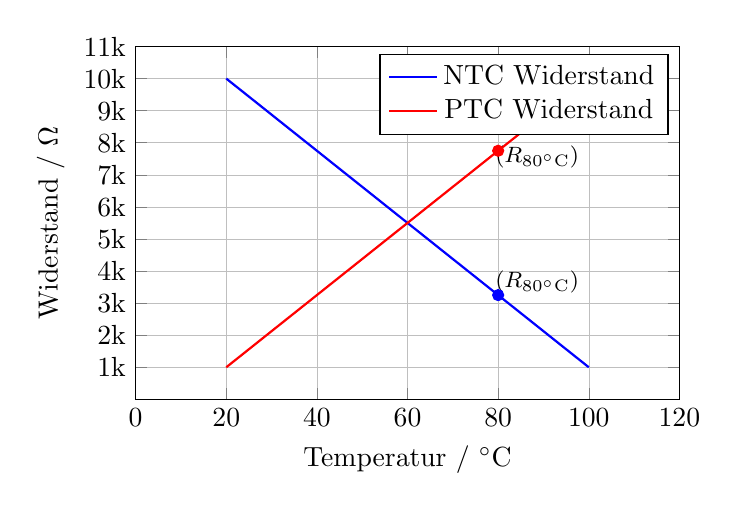
\begin{tikzpicture}
        \begin{axis}[
            xlabel={Temperatur / $^\circ$C},
            ylabel={Widerstand / $\Omega$},
            xmin=0, xmax=120,
            ymin=0, ymax=11000,
            xtick={0,20,...,120},
            ytick={1000,2000,...,11000},
            yticklabels={1k,2k,3k,4k,5k,6k,7k,8k,9k,10k,11k},
            grid=both,
            major grid style={line width=.2pt,draw=gray!50},
            minor grid style={line width=.1pt,draw=gray!20},
            width=0.7\textwidth,
            height=0.5\textwidth,
            scaled y ticks=false
        ]
        
        % NTC Widerstand
        \addplot[
            color=blue,
            mark=none,
            thick,
        ] coordinates {
            (20,10000)(100,1000)
        };
        \addlegendentry{NTC Widerstand}

        % PTC Widerstand
        \addplot[
     	color=red,
		mark=none,
		thick,
	   ] coordinates {
		  (20,1000)(100,10000)
	   };
	   \addlegendentry{PTC Widerstand}

	% Punkte auf der Linie markieren
	\addplot[
		color=red,
		only marks,
		mark=*,
		mark size=2pt
    ]coordinates {
	(80,7750)
	};

    % Punkte auf der Linie markieren
		 \addplot[
          color=blue,
          only marks,
          mark=*,
          mark size=2pt
      ] coordinates {
        (80,3250)
	};

	% Beschriftungen der Punkte PTC
	\node[anchor=south east, font=\footnotesize] at (axis cs:100,6900) {($R_{\mathrm{80^\circ C}}$)};
	% Beschriftungen der Punkte NTC
    \node[anchor=south east, font=\footnotesize] at (axis cs:100,3000) {($R_{\mathrm{80^\circ C}}$)};
        
		\end{axis}
    \end{tikzpicture}
    \s{\caption{\textbf{Diagramm eines linearen NTC- und eines PTC-Widerstands über die Temperatur.} Bei einem NTC sinkt der Widerstand mit steigender Temperatur,
	 während bei einem PTC  der Widerstandswert mit steigender Temperatur ansteigt.}}
    \label{fig:ntc_ptc_widerstandsdiagramm}
\end{figure}
\end{frame}
%%%%%%%%%%%%%%%%%%%%%%%%%%%%%%%%%%%%%%%%%%%%% Ende - Diagramm PTC und NTC %%%%%%%%%%%%%%%%%%%%%%%%%%%%%%%%%%%%
\s{
	Die PTC-Widerstände haben einen positiven Temperaturkoeffizienten $\alpha$, welcher in Tabelle 1 im Abschnitt 1.1.3 abgelesen werden kann. 
	Gut leitfähige Materialien haben ein positives $\alpha$, was bedeutet, dass deren Widerstand bei höheren Temperaturen zunimmt. 
	Somit sind sie im kalten Betrieb leitfähiger, wodurch sie auch "Kaltleiter" genannt werden. 
	In Abbildung \ref{fig:widerstandsdiagramm_ptc} ist der gleiche PTC-Widerstand bei jeweils unterschiedlichen Temperaturen dargestellt.
}

%%%%%%%%%%%%%%%%%%%%%%%%%%%%%%%%%%%%%%%%%%%%% Anfang - Diagramm PTC %%%%%%%%%%%%%%%%%%%%%%%%%%%%%%%%%%%%
\begin{frame}
	\ftx{Temperaturabhängige Widerstände}
	%%% Spannung/ Strom verhältnis über PTC
	\begin{figure}[H]
		\centering
		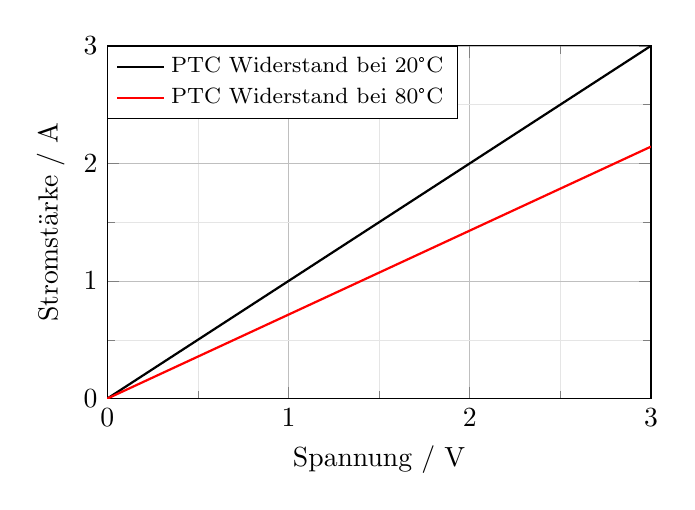
\begin{tikzpicture}
			\begin{axis}[
				xlabel={Spannung / V},
				ylabel={Stromstärke / A},
				xmin=0, xmax=3,
				ymin=0, ymax=3,
				xtick={0,1,2,3},
				ytick={0,1,2,3},
				minor x tick num=1,
				minor y tick num=1,
				grid=both,
				major grid style={line width=.2pt,draw=gray!50},
				minor grid style={line width=.1pt,draw=gray!20},
				legend style={font=\footnotesize, at={(0,1)}, anchor=north west},
				width=0.7\textwidth, % Adjust the width of the plot
				height=0.5\textwidth % Adjust the height of the plot
			]
			
			% Temperaturunabhängiger Widerstand (Steigung 1)
			\addplot[
				color=black,
				mark=none,
				thick,
			] coordinates {
				(0,0)(3,3)
			};
			\addlegendentry{PTC Widerstand bei 20°C}
	
			% Temperaturabhängiger Widerstand (Steigung 1/1.4)
			\addplot[
				color=red,
				mark=none,
				thick,
			] coordinates {
				(0,0)(3,3/1.4)
			};
			\addlegendentry{PTC Widerstand bei 80°C}
	
			\end{axis}
		\end{tikzpicture}
		\s{\caption{Diagramm eines PTC Widerstandes bei 20°C und bei 80°C}
		\label{fig:widerstandsdiagramm_ptc}}
	\end{figure}
\end{frame}
%%%%%%%%%%%%%%%%%%%%%%%%%%%%%%%%%%%%%%%%%%%%% Ende - Diagramm PTC %%%%%%%%%%%%%%%%%%%%%%%%%%%%%%%%%%%%
\s{
	Das folgende Diagramm zeigt die Erwärmung eines PTC-Widerstandes bei Erhöhung des Stromflusses.
	Je mehr Strom also durch einen PTC-Widerstand fließt, desto stärker erwärmt er sich.
}
%%%%%%%%%%%%%%%%%%%%%%%%%%%%%%%%%%%%%%%%%%%%% Anfang - Diagramm Strom - Temperatur Kurve %%%%%%%%%%%%%%%%%%%%%%%%%%%%%%%%%%%%
\begin{frame}
	\ftx{Temperaturabhängige Widerstände}
%%%%% Strom Temperatur verhältnis
\begin{figure}[H]
    \centering
    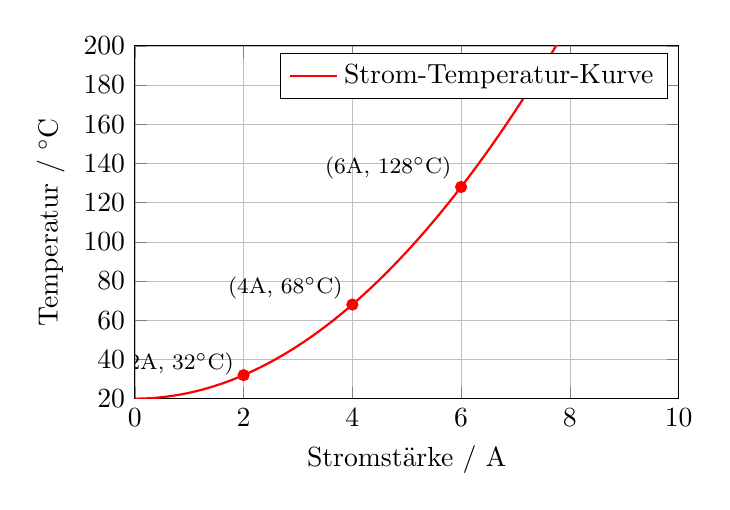
\begin{tikzpicture}
        \begin{axis}[
            xlabel={Stromstärke / A},
            ylabel={Temperatur / $^\circ$C},
            xmin=0, xmax=10,
            ymin=20, ymax=200,
            xtick={0,2,...,10},
            ytick={20,40,...,200},
            grid=both,
            major grid style={line width=.2pt,draw=gray!50},
            minor grid style={line width=.1pt,draw=gray!20},
            width=0.7\textwidth,
            height=0.5\textwidth
        ]
        
        % Plot für Strom-Temperatur-Kurve (nichtlinearer Zusammenhang)
        \addplot[
            color=red,
            domain=0:10,
            samples=100,
            thick,
        ] {20 + x^2 * 3};
        \addlegendentry{Strom-Temperatur-Kurve}
        
        % Markieren von Punkten auf der Linie
        \addplot[
            color=red,
            only marks,
            mark=*,
            mark size=2pt
        ] coordinates {
            (2,32)
            (4,68)
            (6,128)
        };
        
        % Beschriftungen der Punkte
        \node[anchor=south east, font=\footnotesize] at (axis cs:2,27) {($2$A, $32^\circ$C)};
        \node[anchor=south east, font=\footnotesize] at (axis cs:4,66) {($4$A, $68^\circ$C)};
        \node[anchor=south east, font=\footnotesize] at (axis cs:6,127) {($6$A, $128^\circ$C)};
        
        \end{axis}
    \end{tikzpicture}
    \s{\caption{\textbf{Diagramm der Temperatur eines Widerstands in Abhängigkeit von der Stromstärke.} Zeigt wie die Temperatur eines Widerstands
	 mit zunehmender Stromstärke ansteigt. Der Widerstandswert kann sich dabei ebenfalls ändern, abhängig von der Temperaturabhängigkeit des Widerstands.}}
    \label{fig:strom-temperatur}
\end{figure}
\end{frame}
%%%%%%%%%%%%%%%%%%%%%%%%%%%%%%%%%%%%%%%%%%%%% Ende - Diagramm Strom - Temperatur Kurve %%%%%%%%%%%%%%%%%%%%%%%%%%%%%%%%%%%%

\s{
	Das genau entgegengesetzte Verhalten weist ein NTC-Widerstand aufgrund seines negativen Temperaturkoeffizienten auf.
	Typische Materialien mit einem solchen Verhalten sind Grafit oder Silizium. Da diese Widerstände bei zunehmender Temperatur besser leiten, nennt man sie auch Heißleiter.
	In Abbildung \ref{fig:widerstandsdiagramm_ntc} ist zu erkennen, dass der Widerstand
	bei einer höheren Temperatur einen geringeren Widerstandswert aufweist.
}

%%%%%%%%%%%%%%%%%%%%%%%%%%%%%%%%%%%%%%%%%%%%% Anfang - Diagramm NTC %%%%%%%%%%%%%%%%%%%%%%%%%%%%%%%%%%%%
\begin{frame}
	\ftx{Temperaturabhängige Widerstände}
%%% Spannung/ Strom verhältnis über NTC
\begin{figure}[H]
	\centering
	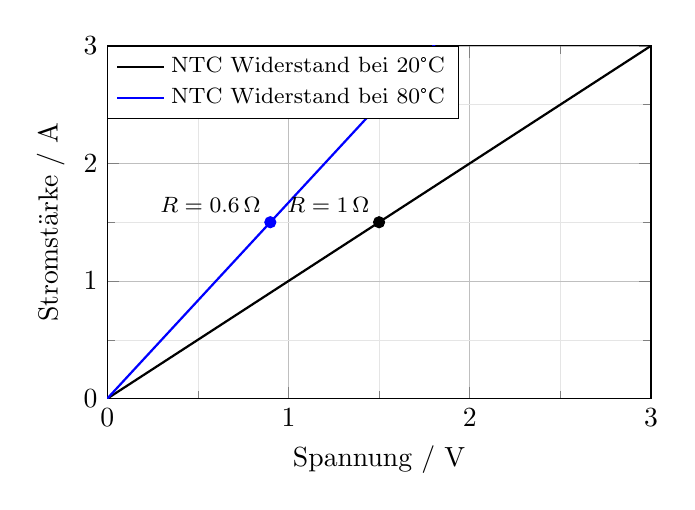
\begin{tikzpicture}
		\begin{axis}[
			xlabel={Spannung / V},
			ylabel={Stromstärke / A},
			xmin=0, xmax=3,
			ymin=0, ymax=3,
			xtick={0,1,2,3},
			ytick={0,1,2,3},
			minor x tick num=1,
			minor y tick num=1,
			grid=both,
			major grid style={line width=.2pt,draw=gray!50},
			minor grid style={line width=.1pt,draw=gray!20},
			legend style={font=\footnotesize, at={(0,1)}, anchor=north west},
			width=0.7\textwidth, % Adjust the width of the plot
			height=0.5\textwidth % Adjust the height of the plot
		]
		
		% Temperaturunabhängiger Widerstand (Steigung 1)
		\addplot[
			color=black,
			mark=none,
			thick,
		] coordinates {
			(0,0)(3,3)
		};
		\addlegendentry{NTC Widerstand bei 20°C}

		% Temperaturabhängiger Widerstand (Steigung 1/1.4)
		\addplot[
			color=blue,
			mark=none,
			thick,
		] coordinates {
			(0,0)(3,3/0.6)
		};
		\addlegendentry{NTC Widerstand bei 80°C}
 % Punkt bei 1.5 A für idealen Widerstand
		\addplot[
			color=black,
			only marks,
			mark=*,
			mark size=2pt
		] coordinates {
			(1.5,1.5)
		};
		\node[anchor=south east, font=\footnotesize] at (axis cs:1.5,1.5) {$R = 1\,\Omega$};
		% Punkt bei 1.5 A für NTC Widerstand
		\addplot[
			color=blue,
			only marks,
			mark=*,
			mark size=2pt
		] coordinates {
			(1.5*0.6,1.5)
		};
		\node[anchor=south east, font=\footnotesize] at (axis cs:0.9,1.5) {$R = 0.6\,\Omega$};
		\end{axis}
	\end{tikzpicture}
	\s{\caption{Diagramm eines NTC Widerstandes bei 20 °C und bei 80 °C}
	\label{fig:widerstandsdiagramm_ntc}}
\end{figure}
\end{frame}
%%%%%%%%%%%%%%%%%%%%%%%%%%%%%%%%%%%%%%%%%%%%% Ende - Diagramm NTC %%%%%%%%%%%%%%%%%%%%%%%%%%%%%%%%%%%%

%%%%%%%%%%%%%%%%%%%%%%%%%%%%%%%%%%%%%%%%%%%%% Ende - PTC und NTC %%%%%%%%%%%%%%%%%%%%%%%%%%%%%%%%%%%%

\newpage	





